
\chapter{ElmerGUI initialization file}

The initialization file for ElmerGUI is located in {\tt ELMERGUI\_HOME/edf}. It is called {\tt egini.xml}:

\begin{footnotesize}
\begin{verbatim}
<?xml version='1.0' encoding='UTF-8'?>
<!DOCTYPE egini>
<egini version="1.0">

  Show splash screen at startup:
  <splashscreen> 1 </splashscreen>

  Show system tray icon:
  <systrayicon> 1 </systrayicon>

  Show system tray messages:
  <systraymessages> 1 </systraymessages>

  System tray message duration in milliseconds:
  <systraymsgduration> 3000 </systraymsgduration>

  Check the presence of external components:
  <checkexternalcomponents> 0 </checkexternalcomponents>

  Hide toolbars:
  <hidetoolbars> 0 </hidetoolbars>

  Plot convergence view:
  <showconvergence> 1 </showconvergence>

  Draw background image:
  <bgimage> 1 </bgimage>

  Background image file:
  <bgimagefile> :/images/bgimage.png </bgimagefile>

  Align background image to the bottom right corner of the screen:
  <bgimagealignright> 0 </bgimagealignright>

  Stretch background image to fit the display area (overrides align):
  <bgimagestretch> 1 </bgimagestretch>

  Maximum number of solvers / equation:
  <max_solvers> 10 </max_solvers>

  Maximum number of equations:
  <max_equations> 10 </max_equations>

  Maximum number of materials:
  <max_materials> 10 </max_materials>

  Maximum number of bodyforces:
  <max_bodyforces> 10 </max_bodyforces>

  Maximum number of initial conditions:
  <max_initialconditions> 10 </max_initialconditions>

  Maximum number of bodies:
  <max_bodies> 100 </max_bodies>

  Maximum number of bcs:
  <max_bcs> 500 </max_bcs>

  Maximum number of boundaries:
  <max_boundaries> 500 </max_boundaries>

</egini>
\end{verbatim}
\end{footnotesize}

You may change the default behavior of ElmerGUI by editing this file. For example, to turn off the splash screen at start up, change the value of the tag {\tt <splshscreen>} from 1 to 0. To change the background image, enter a picture file name in the {\tt <bgimagefile>} tag. You might also want to increase the default values for solvers, equations, etc., in case of very complex models.

\chapter{ElmerGUI material database}

The file {\tt ELMERGUI\_HOME/edf/egmaterials.xml} defines the material database for ElmerGUI. The
format of this file is the following:

\begin{footnotesize}
\begin{verbatim}
 
<!DOCTYPE egmaterials>
<materiallibrary>
  
  <material name="Air (room temperature)" >
    <parameter name="Density" >1.205</parameter>
    <parameter name="Heat conductivity" >0.0257</parameter>
    <parameter name="Heat capacity" >1005.0</parameter>
    <parameter name="Heat expansion coeff." >3.43e-3</parameter>
    <parameter name="Viscosity" >1.983e-5</parameter>
    <parameter name="Turbulent Prandtl number" >0.713</parameter>
    <parameter name="Sound speed" >343.0</parameter>
  </material>

  <material name="Water (room temperature)" >
    <parameter name="Density" >998.3</parameter>
    <parameter name="Heat conductivity" >0.58</parameter>
    <parameter name="Heat capacity" >4183.0</parameter>
    <parameter name="Heat expansion coeff." >0.207e-3</parameter>
    <parameter name="Viscosity" >1.002e-3</parameter>
    <parameter name="Turbulent Prandtl number" >7.01</parameter>
    <parameter name="Sound speed" >1497.0</parameter>
  </material>
  ...
</materiallibrary>

\end{verbatim}
\end{footnotesize}

The values of the parameters may be either constant, or functions of time, temperature, etc.
A temperature dependent parameter may be defined e.g. as

\begin{footnotesize}
\begin{verbatim}
<parameter name="A" >Variable Temperature; Real; 2 3; 4 5; End</parameter>
\end{verbatim}
\end{footnotesize}
In this case, $A(2)=3$ and $A(4)=5$. Values between the points are interpolated linearly,
and extrapolated in the tangent direction outside the domain. The number of points defining 
the interpolant may be arbitrary. 

\chapter{ElmerGUI definition files}

The directory {\tt ELMERGUI\_HOME} contains a subdirectory called ``edf''. This is the place where all ElmerGUI definition files (ed-files) reside. The definition files are XML-formatted text files which define the contents and appearance of the Model menu.

The ed-files are loaded iteratively from the edf-directory once and for all when ElmerGUI starts. Later, it is possible to view and edit their contents by choosing
\menu{File}{Definitions...}

An ed-file has the following structure:
\begin{footnotesize}
\begin{verbatim}
<?xml version='1.0' encoding='UTF-8'?>
<!DOCTYPE edf>
<edf version="1.0">
   [PDE block]
   [PDE block]
   ...
   [PDE block]
</edf>
\end{verbatim}
\end{footnotesize}

The structure of a [PDE block] is the following:
\begin{footnotesize}
\begin{verbatim}
<PDE Name="My equation">
   <Name>
      My equation
   </Name>
   ...
   <Equation>
      [Widget block]
   </Equation>
   ...
   <Material>
      [Widget block]
   </Material>
   ...
   <BodyForce>
      [Widget block]
   <BodyForce>
   ...
   <InitialCondition>
      [Widget block]
   </InitialCondition>
   ...
   <BoundaryCondition>
      [Widget block]
   </BoundaryCondition>
</PDE>
\end{verbatim}
\end{footnotesize}
Note that the name of the PDE is defined redundantly in two occurrences.

The basic structure of a [Widget block] is the following:
\begin{footnotesize}
\begin{verbatim}
<Parameter Widget="Label">
   <Name> My label </Name>
</Parameter>
...
<Parameter Widget="Edit"> 
   <Name> My edit box </Name>
   <Type> Integer </Type>
   <Whatis> Meaning of my edit box </Whatis>
</Parameter>
...
<Parameter Widget="CheckBox">
   <Name> My check box </Name>
   <Type> Logical </Type>
   <Whatis> Meaning of my check box </Whatis>
</Parameter>
...
<Parameter Widget="Combo"> 
   <Name> My combo box </Name> 
   <Type> String </Type>
   <Item> <Name> My 1st item </Name> </Item>
   <Item> <Name> My 2nd item </Name> </Item>
   <Item> <Name> My 3rd item </Name> </Item>
   <Whatis> Meaning of my combo box </Whatis>
</Parameter>
\end{verbatim}
\end{footnotesize}

There are four types of widgets available:
\begin{itemize}
 \item Label (informative text)
 \item CheckBox (switches)
 \item ComboBox (selection from list)
 \item LineEdit (generic variables)
\end{itemize}
Each widget must be given a name and a variable type: logical, integer, real, or  string. It is also a good practice to equip the widgets with tooltips explaining their purpose and meaning as clearly as possible.

Below is a working example of a minimal ElmerGUI definition file. It will add ``My equation'' to the equation tabs in the Model menu, see Figure~\ref{fig_equations}. The file is called ``sample.edf'' and it should be placed in {\tt ELMERGUI\_HOME/edf}.

\begin{footnotesize}
\begin{verbatim}
<?xml version='1.0' encoding='UTF-8'?>
<!DOCTYPE edf>
<edf version="1.0">
  <PDE Name="My equation">
    <Name> My equation </Name>
    <Equation>
      <Parameter Widget="Label">
        <Name> My label </Name>
      </Parameter>
      <Parameter Widget="Edit">
        <Name> My edit box </Name>
        <Type> Integer </Type>
        <Whatis> Meaning of my edit box </Whatis>
      </Parameter>
      <Parameter Widget="CheckBox">
        <Name> My check box </Name>
        <Type> Logical </Type>
        <Whatis> Meaning of my check box </Whatis>	  
      </Parameter>
      <Parameter Widget="Combo">
        <Name> My combo box </Name>
        <Type> String </Type>
        <Item> <Name> My 1st item </Name> </Item>
        <Item> <Name> My 2nd item </Name> </Item>
        <Item> <Name> My 3rd item </Name> </Item>
        <Whatis> Meaning of my combo box </Whatis>	  
      </Parameter>
    </Equation>
  </PDE>
</edf>
\end{verbatim}
\end{footnotesize}

\begin{figure}[htb]
\begin{center}
 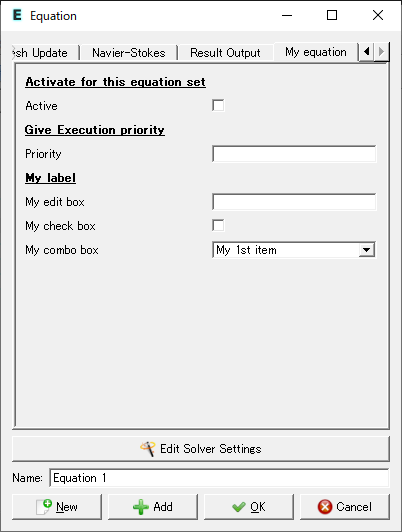
\includegraphics[scale=0.5]{images/edfsample.png}
\caption{Equation tab in Model menu produced by the sample ed-file.}
\label{fig_equations}
\end{center}
\end{figure}

More sophisticated examples with different tags and attributes can be found from the XML-files in  {\tt ELMERGUI\_HOME/edf}.

\newpage

\chapter{Elmer mesh files}

\noindent {\bf mesh.header}
\begin{verbatim}
nodes elements boundary-elements
types
type1 elements1
type2 elements2
...
typeN elementsN
\end{verbatim}

\vskip5mm

\noindent {\bf mesh.nodes}
\begin{verbatim}
node1 tag1 x1 y1 z1
node2 tag2 x2 y2 z2
...
nodeN tagN xN yN zN
\end{verbatim}

\vskip5mm

\noindent {\bf mesh.elements}
\begin{verbatim}
element1 body1 type1 n11 ... n1M
element2 body2 type2 n21 ... n2M
...
elementN bodyN typeN nN1 ... nNM
\end{verbatim}

\vskip5mm

\noindent {\bf mesh.boundary}
\begin{verbatim}
element1 boundary1 parent11 parent12 n11 ... n1M
element2 boundary2 parent21 parent22 n21 ... n2M
...
elementN boundaryN parentN1 parentN2 nN1 ... nNM
\end{verbatim}

\newpage

\chapter{Adding menu entries to ElmerGUI}

As ElmerGUI is based on Qt4, it should be relatively easy to customize the menus
and dialog windows. A new menu item, for example, is added as follows.

First, we declare the menu action and a private slot in {\tt src/mainwindow.h}:
\begin{verbatim}
private slots:
   ...
   void mySlot();
   ...

private:
   ...
   QAction *myAct;
   ...
\end{verbatim}

Then, in {\tt src/mainwindow.cpp}, we actually create the action, connect
an appropriate signal from the action to the slot, and add the action in
a menu:
\begin{verbatim}
void MainWindow::createActions()
{
   ...
   myAct = new QAction(tr("*** My menu entry ***"), this);
   connect(myAct, SIGNAL(triggered()), this, SLOT(mySlot()));
   ...
}
\end{verbatim}
and
\begin{verbatim}
void MainWindow::createMenus()
{
   ...
   meshMenu->addSeparator();
   meshMenu->addAction(myAct);
   ...
}
\end{verbatim}

It finally remains to define the slot to which the triggering signal is connected.
All processing related to the action should be done here:
\begin{verbatim}
void MainWindow::mySlot()
{
   cout << "Here we go!" << endl;
}
\end{verbatim}

\newpage

\chapter{ElmerGUI mesh structure}

The finite element mesh generated by ElmerGUI is of class {\tt mesh\_t}
(declared in {\tt src/meshtype.h}). The mesh is private to the class {\tt GLWidget}
(declared in {\tt src/glwidget.h}), which is responsible of drawing and
rendering the model.

\section{GLWidget}

The class {\tt GLWidget} provides the following public methods for accessing the mesh:
\begin{verbatim}
mesh_t* GLWidget::getMesh()
\end{verbatim}
Get the active mesh.
\begin{verbatim}
void GLWidget::newMesh()
\end{verbatim}
Allocate space for a new mesh.
\begin{verbatim}
void GLWidget::deleteMesh()
\end{verbatim}
Delete the current mesh.
\begin{verbatim}
bool GLWidget::hasMesh()
\end{verbatim}
Returns true if there is a mesh. Otherwise returns false.
\begin{verbatim}
void GLWidget::setMesh(mesh_t* myMesh)
\end{verbatim}
Set active mesh to myMesh.

The mesh can be accessed in {\tt MainWindow} for example as follows
(see previous section for more details):
\begin{verbatim}
void MainWindow::mySlot()
{
   if(!glWidget->hasMesh()) return;
   mesh_t* mesh = glWidget->getMesh();
   cout << "Nodes: " << mesh->getNodes() << endl;
   cout << "Edges: " << mesh->getEdges() << endl;
   cout << "Trias: " << mesh->getSurfaces() << endl;
   cout << "Tetras: " << mesh->getElements() << endl;
}
\end{verbatim}

\section{mesh\_t}

The class {\tt mesh\_t} provides the following public methods for accessing
and manipulating mesh data:
\begin{verbatim}
bool mesh_t::isUndefined()
\end{verbatim}
Returns true if the mesh is undefined. Otherwise returns false.
\begin{verbatim}
void mesh_t::clear()
\end{verbatim}
Clears the current mesh.
\begin{verbatim} 
bool mesh_t::load(char* dir)
\end{verbatim}
Loads Elmer mesh files from directory dir. Returns false if loading failed. Otherwise returns true.
\begin{verbatim} 
bool mesh_t::save(char* dir)
\end{verbatim}
Saves the mesh in Elmer format in directory dir. Returns false if saving failed. Otherwise returns true.
\begin{verbatim} 
double* mesh_t::boundingBox()
\end{verbatim}
Returns bounding box for the current mesh (xmin, xmax, ymin, ymax, zmin, zmax, xmid, ymid, zmid, size).
\begin{verbatim} 
void mesh_t::setCdim(int cdim)
\end{verbatim}
Set coordinate dimension to cdim.
\begin{verbatim}  
int mesh_t::getCdim()
\end{verbatim}
Get coordinate dimension for the current mesh.
\begin{verbatim}  
void mesh_t::setDim(int dim)
\end{verbatim}
Set mesh dimension to dim.
\begin{verbatim}
int mesh_t::getDim()
\end{verbatim}
Get mesh dimension.
\begin{verbatim}  
void mesh_t::setNodes(int n)
\end{verbatim}
Set the number of nodes to n.
\begin{verbatim} 
int mesh_t::getNodes()
\end{verbatim}
Get the number of nodes.
\begin{verbatim} 
void mesh_t::setPoints(int n)
\end{verbatim}
Set the number of point elements to n.
\begin{verbatim} 
int mesh_t::getPoints()
\end{verbatim}
Get the number of point elements.
\begin{verbatim} 
void mesh_t::setEdges(int n)
\end{verbatim}
Set the number of edge elements to n.
\begin{verbatim}   
int mesh_t::getEdges()
\end{verbatim}
Get the number of edge elements.
\begin{verbatim} 
void mesh_t::setSurfaces(int n)
\end{verbatim}
Set the number of surface elements to n.
\begin{verbatim} 
int mesh_t::getSurfaces()
\end{verbatim}
Get the number of surface elements.
\begin{verbatim} 
void mesh_t::setElements(int n)
\end{verbatim}
Set the number of volume elements to n.
\begin{verbatim} 
int mesh_t::getElements()
\end{verbatim}
Get the number of volume elements.
\begin{verbatim} 
node_t* mesh_t::getNode(int n)
\end{verbatim}
Get node n.
\begin{verbatim} 
void mesh_t::setNodeArray(node_t* nodeArray)
\end{verbatim}
Set node array point to nodeArray. Useful, if the user wants to take care of memory allocation by him/her self.
\begin{verbatim} 
void mesh_t::newNodeArray(int n)
\end{verbatim}
Allocate memory for n nodes.
\begin{verbatim}
void mesh:t::deleteNodeArray()
\end{verbatim}
Delete current node array.
\begin{verbatim}
point_t* mesh_t::getPoint(int n)
\end{verbatim}
Get point element n.
\begin{verbatim}
void mesh_t::setPointArray(point_t* pointArray)
\end{verbatim}
Set point element array point to pointArray. Useful, if the user wants to take care of memory allocation by him/her self.
\begin{verbatim} 
void mesh_t::newPointArray(int n)
\end{verbatim}
Allocate memory for n point elements.
\begin{verbatim}
void mesh_t::deletePointArray()
\end{verbatim}
Delete current point element array.
\begin{verbatim}
edge_t* mesh_t::getEdge(int n)
\end{verbatim}
Get edge element n.
\begin{verbatim}
void mesh_t::setEdgeArray(edge_t* edgeArray)
\end{verbatim}
Set edge element array point to edgeArray. Useful, if the user wants to take care of memory allocation by him/her self.
\begin{verbatim} 
void mesh_t::newEdgeArray(int n)
\end{verbatim}
Allocate memory for n edge elements.
\begin{verbatim}
void mesh_t::deleteEdgeArray()
\end{verbatim}
Delete current edge element array.
\begin{verbatim}
surface_t* mesh_t::getSurface(int n)
\end{verbatim}
Get surface element n.
\begin{verbatim}
void mesh_t::setSurfaceArray(surface_t* surfaceArray)
\end{verbatim}
Set surface element array point to surfaceArray. Useful, if the user wants to take care of memory allocation by him/her self.
\begin{verbatim} 
void mesh_t::newSurfaceArray(int n);
\end{verbatim}
Allocate memory for n surface elements.
\begin{verbatim}
void mesh_t::deleteSurfaceArray()
\end{verbatim}
Delete surface element array.
\begin{verbatim}
element_t* mesh_t::getElement(int n)
\end{verbatim}
Get volume element n.
\begin{verbatim}
void mesh_t::setElementArray(element_t* elementArray)
\end{verbatim}
Set volume element array point to elementArray. Useful, if the user wants to take care of memory allocation by him/her self.
\begin{verbatim} 
void mesh_t::newElementArray(int n)
\end{verbatim}
Allocate memory for n volume elements.
\begin{verbatim} 
void mesh_t::deleteElementArray()
\end{verbatim}
Delete current volume element array.

\section{node\_t}

The class {\tt node\_t} has been declared in {\tt src/meshtypes.h}. It provides the
following public methods for accessing node data:
\begin{verbatim}
void node_t::setX(int n, double x)
\end{verbatim}
Set component n of the position vector to x.
\begin{verbatim} 
double node_t::getX(int n)
\end{verbatim}
Get component n of the position vector.
\begin{verbatim} 
void node_t::setXvec(double* v)
\end{verbatim}
Set the position vector to v.
\begin{verbatim} 
double* node_t::getXvec()
\end{verbatim}
Get the position vector.
\begin{verbatim}
void node_t::setIndex(int n)
\end{verbatim}
Set the index of the node to n.
\begin{verbatim} 
int node_t::getIndex()
\end{verbatim}
Get the index of the node.

\section{Base element class element\_t}

The class {\tt element\_t} provides the following methods for accessing element data:
\begin{verbatim} 
void element_t::setNature(int n)
\end{verbatim}
Set element nature to n (either PDE\_UNKNOWN, PDE\_BOUNDARY, or PDE\_BULK).
\begin{verbatim}
int element_t::getNature()
\end{verbatim}
Get the element nature.
\begin{verbatim}
void element_t::setCode(int n)
\end{verbatim}
Set element code to n (202 = two noded line, 303 = three noded triangle, ...)
\begin{verbatim}
int element_t::getCode()
\end{verbatim}
Get the element code.
\begin{verbatim}
void element_t::setNodes(int n)
\end{verbatim}
Set the number of nodes to n.
\begin{verbatim}
int element_t::getNodes()
\end{verbatim}
Get the number of nodes.
\begin{verbatim}
void element_t::setIndex(int n)
\end{verbatim}
Set element index to n.
\begin{verbatim}
int element_t::getIndex()
\end{verbatim}
Get the element index.
\begin{verbatim}
void element_t::setSelected(int n)
\end{verbatim}
Set the selection state (1=selected, 0=unselected).
\begin{verbatim}
int element_t::getSelected()
\end{verbatim}
Returns 1 if element is selected. Otherwise returns 0.
\begin{verbatim}
int element_t::getNodeIndex(int n)
\end{verbatim}
Get the index of node n.
\begin{verbatim}
void element_t::setNodeIndex(int m, int n)
\end{verbatim}
Set the index of node m to n.
\begin{verbatim}
int* element_t::getNodeIndexes()
\end{verbatim}
Get the indexes of all nodes.
\begin{verbatim}
void element_t::newNodeIndexes(int n)
\end{verbatim}
Allocate space for n node indexes.
\begin{verbatim}
void element_t::deleteNodeIndexes()
\end{verbatim}
Delete all node indexes.

\section{Point element class point\_t}

The class {\tt point\_t} inherits all public members from class {\tt element\_t}.
In addition to this, it provides the following methods for accessing and
manipulating point element data:
\begin{verbatim}
void setSharp(bool b);
\end{verbatim}
Mark the point element ``sharp'' (b=true) or not (b=false).
\begin{verbatim}
bool isSharp();
\end{verbatim}
Returns true if the point element is ``sharp''. Otherwise returns false.
\begin{verbatim}
void setEdges(int n);
\end{verbatim}
Set the number of edges elements connected to the point to n.
\begin{verbatim}
int getEdges();
\end{verbatim}
Get the number of edge elements connected to the point.
\begin{verbatim}
void setEdgeIndex(int m, int n);
\end{verbatim}
Set the index of m'th edge element to n.
\begin{verbatim}
int getEdgeIndex(int n);
\end{verbatim}
Get the index of n'th connected edge element.
\begin{verbatim}
void newEdgeIndexes(int n);
\end{verbatim}
Allocate space for n edge element indexes.
\begin{verbatim}
void deleteEdgeIndexes();
\end{verbatim}
Delete all edge element indexes.

\section{Edge element class edge\_t}

The class {\tt edge\_t} inherits all public methods from {\tt element\_t}.
It also provides the following methods for accessing and manipulating edge
element data:
\begin{verbatim}
void edge_t::setSharp(bool b)
\end{verbatim}
Mark the edge sharp (b=true) or not (b=false).
\begin{verbatim}
bool edge_t::isSharp()
\end{verbatim}
Returns true if the edge is sharp.
\begin{verbatim} 
void edge_t::setPoints(int n)
\end{verbatim}
Set the number of point elements connected to the edge to n.
\begin{verbatim}
int edge_t::getPoints()
\end{verbatim}
Get the number of point elements connected to the edge.
\begin{verbatim}
void edge_t::setPointIndex(int m, int n)
\end{verbatim}
Set the index of point element m to n.
\begin{verbatim}
int edge_t::getPointIndex(int n)
\end{verbatim}
Get the index of point element n.
\begin{verbatim}
void edge_t::newPointIndexes(int n)
\end{verbatim}
Allocate space for n point element indexes.
\begin{verbatim}
void edge_t::deletePointIndexes()
\end{verbatim}
Delete all point element indexes.
\begin{verbatim}
void edge_t::setSurfaces(int n)
\end{verbatim}
Set the number of surface elements connected to the edge to n.
\begin{verbatim}
int edge_t::getSurfaces()
\end{verbatim}
Get the number of surface elements connected to the edge.
\begin{verbatim}
void edge_t::setSurfaceIndex(int m, int n)
\end{verbatim}
Set the index of surface element m to n.
\begin{verbatim}
int edge_t::getSurfaceIndex(int n)
\end{verbatim}
Get the index of m'th surface element connected to the edge.
\begin{verbatim}
void edge_t::newSurfaceIndexes(int n)
\end{verbatim}
Allocate space for n surface element indexes.
\begin{verbatim}
void edge_t::deleteSurfaceIndexes()
\end{verbatim}
Delete all surface element indexes.

\section{Surface element class surface\_t}

Finally, the class {\tt surface\_t} provides the following public methods for
accessing and manipulating surface element data, besides of those inherited
from the base element class {\tt element\_t}:

\begin{verbatim}
void surface_t::setEdges(int n)
\end{verbatim}
Set the number of edge elements connected to the surface to n.
\begin{verbatim}
int surface_t::getEdges()
\end{verbatim}
Get the number of edge elements connected to the surface element.
\begin{verbatim}
void surface_t::setEdgeIndex(int m, int n)
\end{verbatim}
Set the index of m'th edge element to n.
\begin{verbatim}
int surface_t::getEdgeIndex(int n)
\end{verbatim}
Get the index of n'th edge element connected to the surface element.
\begin{verbatim}
void surface_t::newEdgeIndexes(int n)
\end{verbatim}
Allocate space for n edge element indexes.
\begin{verbatim}
void surface_t::deleteEdgeIndexes()
\end{verbatim}
Delete all edge element indexes.
\begin{verbatim}
void surface_t::setElements(int n)
\end{verbatim}
Set the number of volume elements connected to the surface element to n.
\begin{verbatim}
int surface_t::getElements()
\end{verbatim}
Get the number of volume elements connected to the surface element.
\begin{verbatim}
void surface_t::setElementIndex(int m, int n)
\end{verbatim}
Set the index of m'th volume element to n.
\begin{verbatim}
int surface_t::getElementIndex(int n)
\end{verbatim}
Get the index of n'th volume element connected to the surface.
\begin{verbatim}
void surface_t::newElementIndexes(int n)
\end{verbatim}
Allocate space for n volume element indexes.
\begin{verbatim}
void surface_t::deleteElementIndexes()
\end{verbatim}
Delete all volume element indexes.
\begin{verbatim}
void surface_t::setNormalVec(double* v)
\end{verbatim}
Set the normal vector to the surface element.
\begin{verbatim}
double* surface_t::getNormalVec()
\end{verbatim}
Get the normal vector for the surface element.
\begin{verbatim}
double surface_t::getNormal(int n)
\end{verbatim}
Get component n of the normal vector.
\begin{verbatim}
void surface_t::setNormal(int n, double x)
\end{verbatim}
Set component n of the normal to x.
\begin{verbatim}
void surface_t::setVertexNormalVec(int n, double* v)
\end{verbatim}
Set the normal vector for vertex n to v.
\begin{verbatim}
void surface_t::addVertexNormalVec(int m, double* v)
\end{verbatim}
Add vector v to the normal in vertex n.
\begin{verbatim}
void surface_t::subVertexNormalVec(int m, double* v)
\end{verbatim}
Subtract vector v from the normal in vertex n.
\begin{verbatim}
double* surface_t::getVertexNormalVec(int n)
\end{verbatim}
Get the normal vector in vertex n.

